\documentclass[12pt]{article}
\usepackage{amsfonts, epsfig}
\usepackage[authoryear]{natbib}
\usepackage{array}
\usepackage{multirow}
\usepackage{graphicx}
\usepackage{fancyhdr}
\usepackage{amsmath}
\usepackage{amssymb}
\pagestyle{fancy}
\lfoot{\texttt{semtm0051.github.io} }
\lhead{Beyond all-to-all - Conor}
\rhead{\thepage}
\cfoot{}

\usepackage{tikz}
\usetikzlibrary{positioning}
\usetikzlibrary{decorations.pathreplacing, calc}
\usetikzlibrary{arrows.meta}

\NewDocumentCommand{\onslide}{d<>}{} % cheating for code carried over from the slides!

\usepackage{ifthen}
\newboolean{nopics}
\setboolean{nopics}{true}


\begin{document}

\section*{Beyond all-to-all!} 


So far all the networks we have looked at have been ``all to all'',
every node from one layer is connected to each layer in the next, as
in Fig.~\ref{fig:all-to-all}.  This is obviously nicely simple but it
clearly fails to exploit the structure of data.  In this lecture we
will look at some of these novel architectures, emphasising this
story: progress has been made by moving away from all-to-all networks
while retaining trust in the power of neural networks.


\begin{figure}[b]
\begin{center}
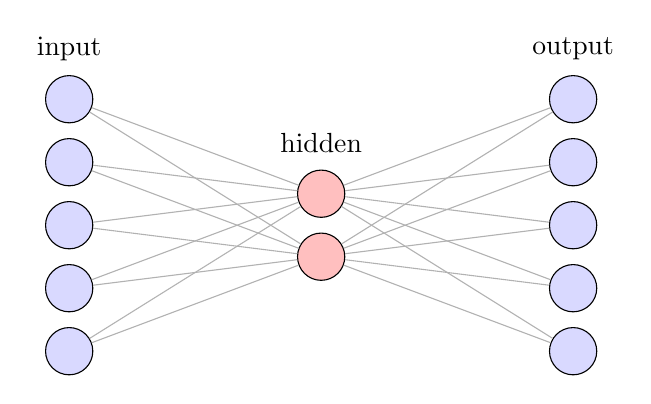
\begin{tikzpicture}[
    neuron/.style={circle,draw,minimum size=6mm,inner sep=0pt},
    edge/.style={gray!60},
    x=1.6cm,y=0.8cm]

  % input layer
  \foreach \i in {1,...,5}
    \node[neuron,fill=blue!15] (x\i) at (0,3-\i) {};

  % bottleneck
  \foreach \i in {1,2}
    \node[neuron,fill=red!25] (z\i) at (2,1.5-\i) {};

  % output layer
  \foreach \i in {1,...,5}
    \node[neuron,fill=blue!15] (y\i) at (4,3-\i) {};

  % connections
  \foreach \i in {1,...,5}
    \foreach \j in {1,2} {
      \draw[edge] (x\i) -- (z\j);
      \draw[edge] (z\j) -- (y\i);
    }

  % labels
  \node at (0,2.8)  {input};
  \node at (2,1.3)  {hidden};
  \node at (4,2.8)  {output};

\end{tikzpicture}
\end{center}
\caption{A cartoon of an all-to-all network. \label{fig:all-to-all}}
\end{figure}




\subsection*{A little historical context}

The history of machine learning has seen a lot of variation in how
much we have tried to design or craft the components of a machine
learning system. At various times in the past people have been
optimistic that a sort of universal principle of computation could
make inferential machines easy to design, without components tailored
to the data the system is dealing with.

The first of these periods came in the late 1950s with Rosenblatt's
perceptron, a simple network of threshold units with a learning rule
that was guaranteed to find a solution whenever one existed; for a
while it seemed as if any problem of perception might yield to the
same device, until Minsky and Papert showed in 1969 that there were
quite simple things, such as deciding whether two inputs differ, that
a single layer could never represent. The second came in the
mid-1980s, when backpropagation gave a way to train networks with
hidden layers, removing the Minsky and Papert limitation, and when,
soon afterwards, the universal approximation theorems showed that a
network with a single hidden layer, each unit connected to every
input, could approximate any reasonable function to arbitrary
accuracy: the all-to-all network, along with a general-purpose
learning rule, appeared to be all that was needed. In both cases the
optimism was more than the results deserved, since knowing that a network can
represent a function says very little about whether it can learn that
function from a realistic amount of data.

In fact, one consequence of the universal approximation theorems was a
widespread belief that there was little point in making networks deep:
if a single hidden layer could already approximate any function, then
extra layers seemed to add nothing except difficulty, and the
difficulty was real, since the gradients that backpropagation relies
on tend to shrink or blow up as they pass back through many layers, so
that deep networks were in practice very hard to train. What was
missing was any expectation that depth might matter for learning
rather than for representation; the theorems say that a suitable
shallow network exists, but they are silent about how wide it needs to
be, which can be astronomically wide, and about whether it can be
found from data, whereas a deep network can build a complicated
function by composing simple ones, reusing at each layer what was
worked out at the layer before.

Anyway, all this meant that the 90s and the very early 2000s were
spent on very bespoke approaches to data, support vector machines,
kernel methods and graphical approaches represented a sort of
unromantic approach to artificial intelligence. The idea was that
there was no `magic' in machine learning, you got out what you put it,
if you wanted to perform inference on data you had to have a
well-understood, unambitious approach to understanding it. This
represented a lot of careful work that produced incremental progress,
and proposed complex multi-component algorithms for processing complex
data, often based on an intricate workflow with different
hand-designed stages.  A lot of this was swept away with the
deep-learning revolution, the practitioners all jumped ship ten years
ago or became grumpy old folk trying to pick holes in neural networks,
muttering `they are just stochastic parrots, now get off my lawn' and
that sort of thing.

Of course, the unromantic approach never completely took over, there
was a heretical group of neural network enthusiasts, Hinton, LeCun,
Bengio and their students; people who knew a bit of neuroscience and
believed in neural computation, who kept working on neural
networks. They believed that the basic ideas, networks,
back-propagation, where good ones but they needed a few extra
ingredients and perhaps a little more stucture, something more bespoke
than all-to-all networks but less tailored than the complicated
schemes that were in fashion then. They wanted to give over to the
unreasonable effectiveness of neural networks what networks could do
well, even if we don't fully understand what they are doing, while
adding a bit of structure and engineering insight. Ultimately, armed
with lots of data, a bag of tricks, the understand that deep networks
are better at learning the structure of data and with the extra speed
from GPUs, they were proved correct in they were proved correct in
2012, when AlexNet, a deep convolutional network trained on GPUs, won
the ImageNet image classification challenge by a margin that left
little room for argument.

\subsection*{Convolutional neural networks}

We tend to forget, but before GPT2 a lot of the focus in machine
learning was on vision, image recognition and even image
generation. These days we are thinking a lot about images again, but
in the context of multi-modal machines that link images in to language
models; at the start of the deep-learning revolution the progress was
being made in pure vision models.

\begin{figure}
\begin{center}
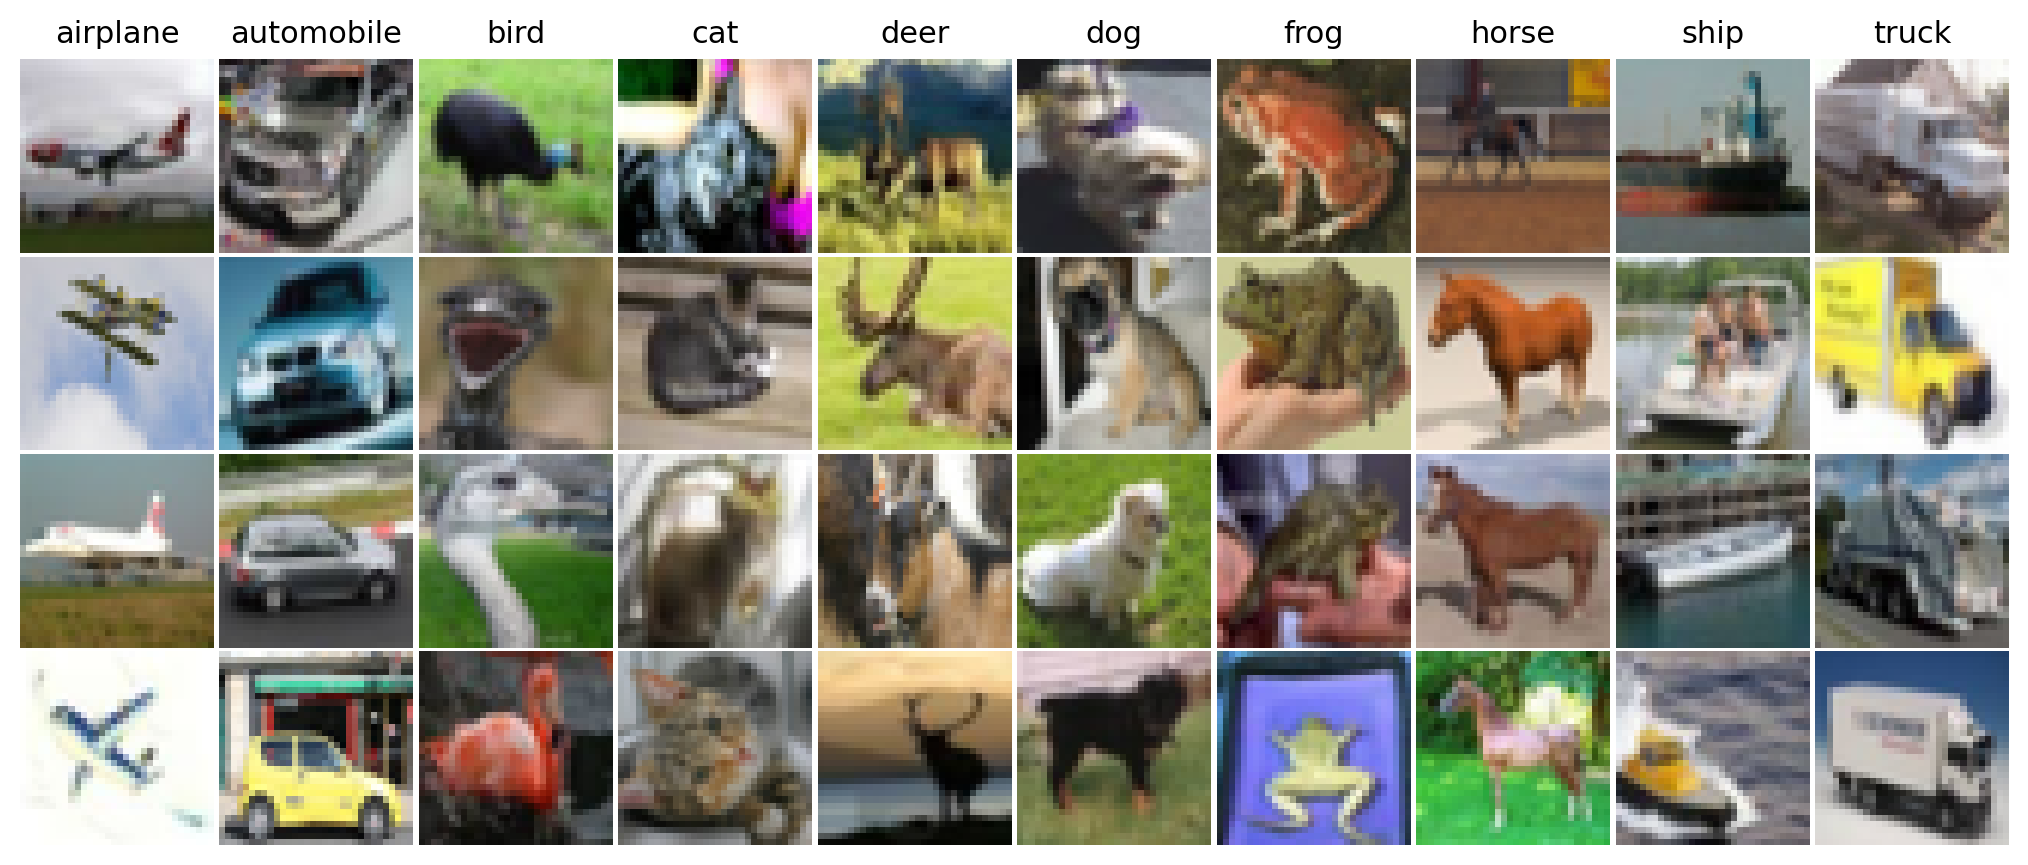
\includegraphics[width=0.9\textwidth]{cifar_grid.png}
\end{center}
\caption{Example CIFAR images, harder and more useful than MNIST, but still a simple classification task. A truck is like a lorry but bigger. \label{fig:cifar}}
\end{figure}

To give some context a common challenge was the CIFAR-10 dataset,
sixty thousand tiny colour images, $32\times32$ pixels, in ten
classes: airplane, automobile, bird, cat, deer, dog, frog, horse,
ship, truck. That's 6,000 per class, split 50,000 for training and
10,000 for testing (Krizhevsky, 2009), examples are shown in
Fig.~\ref{fig:cifar}. As a vector each image is just
$32\times32\times3=3072$ numbers, and the cat can be anywhere in the
frame, any size, facing any way, against any background.

One intuitive idea is that the classification of the image is the end point of a sort of hierarchy:
\begin{center}
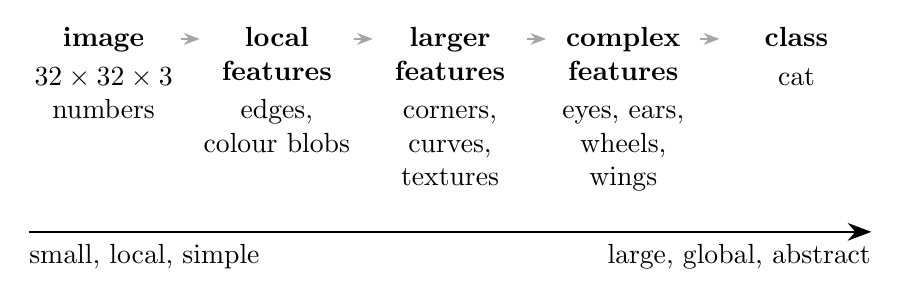
\begin{tikzpicture}[
    stage/.style={align=center,text width=1.9cm,inner sep=0pt,anchor=north},
    arr/.style={-{Stealth[length=2mm]},thick,gray!70}]

  % centres 2.2cm apart; arrows sit level with the first (bold) line
  \node[stage] (s0) at (0,0) {\textbf{image}\\[2pt] $32\times32\times3$ numbers};
  \onslide<2->{
  \node[stage] (s1) at (2.2,0) {\textbf{local features}\\[2pt] edges, colour blobs};
  \draw[arr] (0.98,-0.15) -- (1.22,-0.15);}
  \onslide<3->{
  \node[stage] (s2) at (4.4,0) {\textbf{larger features}\\[2pt] corners, curves, textures};
  \draw[arr] (3.18,-0.15) -- (3.42,-0.15);}
  \onslide<4->{
  \node[stage] (s3) at (6.6,0) {\textbf{complex features}\\[2pt] eyes, ears, wheels, wings};
  \draw[arr] (5.38,-0.15) -- (5.62,-0.15);}
  \onslide<5->{
  \node[stage] (s4) at (8.8,0) {\textbf{class}\\[2pt] cat};
  \draw[arr] (7.58,-0.15) -- (7.82,-0.15);}

  \onslide<6->{
  \draw[-{Stealth[length=3mm]},thick] (-0.95,-2.6) -- (9.75,-2.6);
  \node[anchor=north west,inner sep=0pt] at (-0.95,-2.75) {small, local, simple};
  \node[anchor=north east,inner sep=0pt] at (9.75,-2.75) {large, global, abstract};}
\end{tikzpicture}
\end{center}
In this scheme the network will `build up' its idea of what the image
is of by moving from towards higher and higher level concepts, it
starts with basic local stuff, edges and blobs, areas of colour, in
the next stage it ties them together to form more complicated shapes
and still larger, most specific shapes and even components likes eyes
or wheels before putting recognizing the image as a whole. In this
scheme each stage only looks at a small neighbourhood of the stage
before, but because the stages stack, what each unit ``sees'' of the
original image grows as we go up.

\begin{figure}
\centering
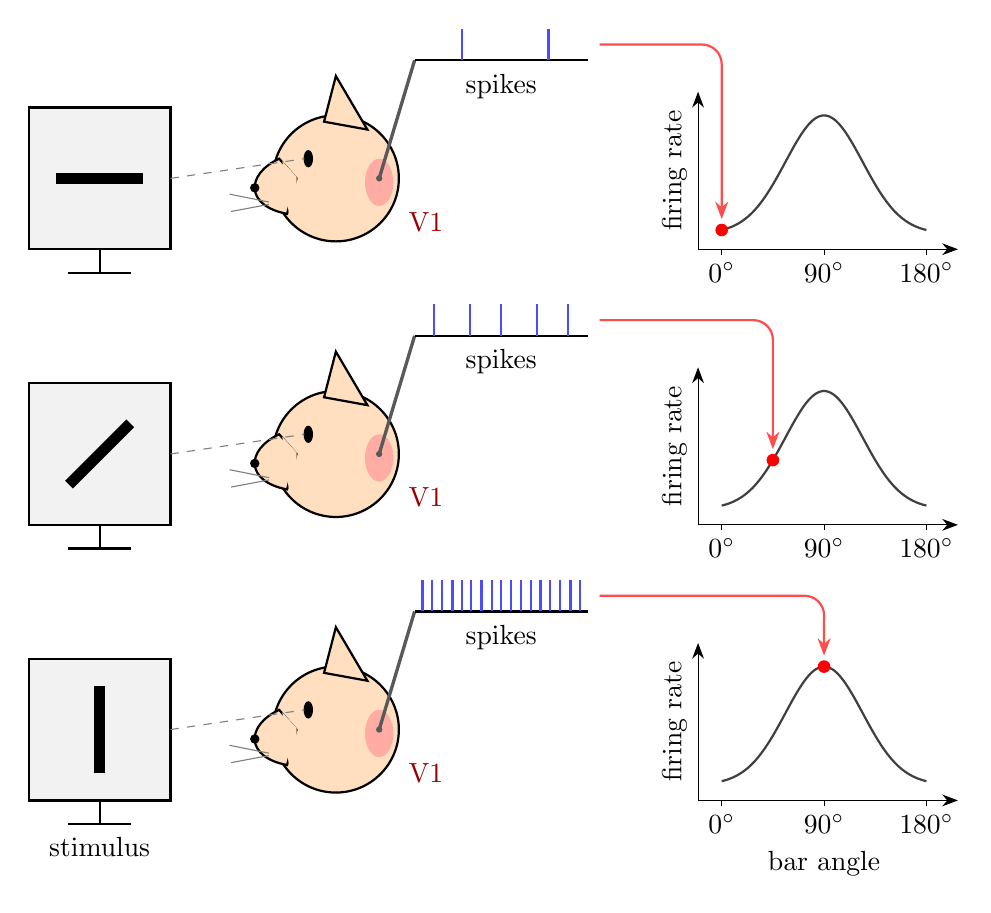
\begin{tikzpicture}[spike/.style={thick,blue!70}]
\foreach \row/\ang/\dx/\dy/\spk in {%
  0/0/0.3/0.244/{0.6,1.7},
  1/45/0.95/0.822/{0.25,0.7,1.1,1.55,1.95},
  2/90/1.6/1.7/{0.1,0.22,0.35,0.48,0.6,0.72,0.85,0.98,1.1,1.22,1.35,1.48,1.6,1.72,1.85,1.98,2.1}}
{
\begin{scope}[shift={(0,{-3.5*\row})}]

  % ---------------- screen with bar
  \draw[thick,fill=gray!10] (-0.9,-0.9) rectangle (0.9,0.9);
  \draw[thick] (0,-0.9) -- (0,-1.2);
  \draw[thick] (-0.4,-1.2) -- (0.4,-1.2);
  \fill[black,rotate around={\ang:(0,0)}] (-0.55,-0.07) rectangle (0.55,0.07);
  \ifnum\row=2 \node[below] at (0,-1.25) {stimulus};\fi

  % ---------------- cat head in profile, facing left
  \begin{scope}[shift={(3.0,0)}]
    \fill[orange!25,draw=black,thick] (0,0) circle (0.8);
    \fill[orange!25,draw=black,thick] (-0.15,0.72) -- (0.0,1.3) -- (0.4,0.62) -- cycle;
    \fill[orange!25,draw=black,thick] (-0.62,-0.45) .. controls (-1.15,-0.35) and (-1.15,0.05) .. (-0.72,0.25)
          -- (-0.5,0) -- cycle;
    \fill[black] (-1.03,-0.12) circle (0.06);
    \fill[black] (-0.35,0.25) ellipse (0.06 and 0.11);
    \draw[gray] (-0.85,-0.3) -- (-1.35,-0.2) (-0.85,-0.33) -- (-1.33,-0.42);
    \fill[orange!25] (-0.5,-0.42) -- (-0.5,0.02) -- (-0.68,0.22) -- (-0.6,-0.43) -- cycle;
    \fill[red!40,opacity=0.7] (0.55,-0.05) ellipse (0.18 and 0.3);
    \draw[very thick,gray!70!black] (0.55,0.0) -- (1.0,1.5);
    \fill[gray!70!black] (0.55,0.0) circle (0.04);
    \node[anchor=west,red!60!black] at (0.8,-0.55) {V1};
  \end{scope}

  % sight line
  \draw[dashed,gray] (0.9,0) -- (2.6,0.25);

  % ---------------- spike recording
  \begin{scope}[shift={(4.0,1.5)}]
    \draw[thick] (0,0) -- (2.2,0);
    \foreach \t in \spk \draw[spike] (\t,0) -- (\t,0.4);
    \node[anchor=north] at (1.1,-0.05) {spikes};
  \end{scope}

  % ---------------- tuning curve
  \begin{scope}[shift={(7.6,-0.9)}]
    \draw[-{Stealth[length=2mm]}] (0,0) -- (3.3,0);
    \draw[-{Stealth[length=2mm]}] (0,0) -- (0,2.0);
    \node[rotate=90] at (-0.3,1.0) {firing rate};
    \foreach \x/\l in {0.3/0^\circ,1.6/90^\circ,2.9/180^\circ}{
      \draw (\x,0) -- (\x,-0.07);
      \node[below] at (\x,-0.05) {$\l$};}
    \ifnum\row=2 \node at (1.6,-0.8) {bar angle};\fi
    \draw[thick,gray!50!black,domain=0.3:2.9,samples=60,smooth]
      plot (\x,{0.2+1.5*exp(-((\x-1.6)^2)/(2*0.49^2))});
    \fill[red] (\dx,\dy) circle (0.08);
    \coordinate (dot) at (\dx,\dy);
  \end{scope}

  % ---------------- arrow from the spikes to the dot
  \draw[-{Stealth[length=2.2mm]},thick,red!70,rounded corners=2.5mm]
    (6.35,1.7) -| ([yshift=1.4mm]dot);

\end{scope}
}
\end{tikzpicture}
\caption{Hubel and Wiesel (1959) recorded single neurons in the visual
  cortex of anaesthetised cats: each cell fires for a bar at one
  orientation, in one small patch of the visual field. If the bar was somewhere else it wouldn't cause neural activity in that particular cell and the activity it causes depends on orientation. This is very much a schematic but if you look around for it there is a film of them performing the original experiment. \label{fig:h7w}}
\end{figure}

This was widely believed to be the scheme used in the brain! In the
late fifties Hubel and Wiesel performed a series of experiments using
anaesthetised cats, using electrodes they recorded the activity of
cells in the primary visual cortex, the part of the brain that deals
with images in a fairly raw form. This is, perhaps surprisingly, at
the back of the brain, as far from the eye as it could easily be; the
visual signal has come from the eye and gone through thalamus where it
undergoes some denoising and adjustment to correct for overall
brightness, the signal then goes to visual cortex.

In the primary visual cortex there there are cells, called simple
cells, that respond to the input in the way illustrated in
Fig.~\ref{fig:h7w}; the visual cortex in many mammals, certainly is
lots of mammals that hunt and have eyes on the front, or front-ish, of
their head, is arranged topographically, different parts deal with
different parts of the visual field and they are laid out sort of
logically, with nearby cells corresponding to nearby parts of the
field. These cells seem to be activated by edges, and are arranged in
a circle, often called a pinwheel, for each location in the field, as
you go around the pinwheel the prefered direction of the edge
rotates. In this way the primary visual cortex seems to do just what
we imagined above, it goes beyond the individual pixes, in this case
the denoised and mildly aggregated inputs from individual retinal
cells and finds local features and there is a mathematical
explaination why edges are the right thing to code for.

The rest of the story seems to sort of hold, cells along the visual
pathway respond to more complex shapes and there are eventually cells
that respond to specific objects; however, as with anything in the
brain, this version of the story turns out to be complicated and, of
course, we need to bear in mind that the brain isn't a deep network;
it only takes a few hundred milliseconds to recognize things and at
the speed the brain operates, this does allow for a huge number of
layers.




\end{document}
